\question[3]
Bestimme für den Graphen einen minimalen Spannbaum mit dem Algorithmus von Jarnik-Prim. Immer wenn der Algorithmus uns eine
Wahl lässt, wählen wir in alphabetischer Reihenfolge. Das bedeutet u.a., dass wir von Knoten a aus starten.

Gib die Kanten in der Reihenfolge an, in der sie gewählt werden. und die Kosten des MST an.


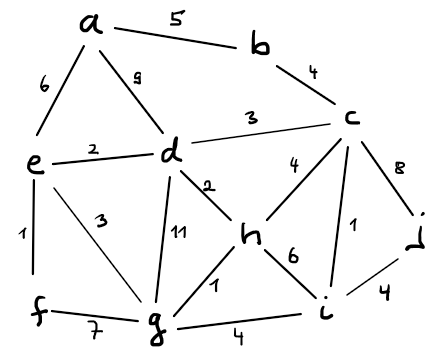
\includegraphics[height=5cm]{\pfad/Graphen/Aufgaben/prim_03/prim_03.png}
\begin{solutionbox}{3cm}
\begin{lstlisting}
a-b, b-c, c-i, c-d, d-e, e-f, d-h, h-g, i-j
Gesamtkosten:  23
\end{lstlisting}
\end{solutionbox}
